%% fcup-thesis.tex -- document template for PhD theses at FCUP
%%
%% Copyright (c) 2015 João Faria <joao.faria@astro.up.pt>
%%
%% This work may be distributed and/or modified under the conditions of
%% the LaTeX Project Public License, either version 1.3c of this license
%% or (at your option) any later version.
%% The latest version of this license is in
%%     http://www.latex-project.org/lppl.txt
%% and version 1.3c or later is part of all distributions of LaTeX
%% version 2005/12/01 or later.
%%
%% This work has the LPPL maintenance status "maintained".
%%
%% The Current Maintainer of this work is
%% João Faria <joao.faria@astro.up.pt>.
%%
%% This work consists of the files listed in the accompanying README.

%% SUMMARY OF FEATURES:
%%
%% All environments, commands, and options provided by the `ut-thesis'
%% class will be described below, at the point where they should appear
%% in the document.  See the file `ut-thesis.cls' for more details.
%%
%% To explicitly set the pagestyle of any blank page inserted with
%% \cleardoublepage, use one of \clearemptydoublepage,
%% \clearplaindoublepage, \clearthesisdoublepage, or
%% \clearstandarddoublepage (to use the style currently in effect).
%%
%% For single-spaced quotes or quotations, use the `longquote' and
%% `longquotation' environments.


%%%%%%%%%%%%         PREAMBLE         %%%%%%%%%%%%

%%  - Default settings format a final copy (single-sided, normal
%%    margins, one-and-a-half-spaced with single-spaced notes).
%%  - For a rough copy (double-sided, normal margins, double-spaced,
%%    with the word "DRAFT" printed at each corner of every page), use
%%    the `draft' option.
%%  - The default global line spacing can be changed with one of the
%%    options `singlespaced', `onehalfspaced', or `doublespaced'.
%%  - Footnotes and marginal notes are all single-spaced by default, but
%%    can be made to have the same spacing as the rest of the document
%%    by using the option `standardspacednotes'.
%%  - The size of the margins can be changed with one of the options:
%%     . `narrowmargins' (1 1/4" left, 3/4" others),
%%     . `normalmargins' (1 1/4" left, 1" others),
%%     . `widemargins' (1 1/4" all),
%%     . `extrawidemargins' (1 1/2" all).
%%  - The pagestyle of "cleared" pages (empty pages inserted in
%%    two-sided documents to put the next page on the right-hand side)
%%    can be set with one of the options `cleardoublepagestyleempty',
%%    `cleardoublepagestyleplain', or `cleardoublepagestylestandard'.
%%  - Any other standard option for the `report' document arclass can be
%%    used to override the default or draft settings (such as `10pt',
%%    `11pt', `12pt'), and standard LaTeX packages can be used to
%%    further customize the layout and/or formatting of the document.

%% *** Add any desired options. ***
%PDF
%\documentclass[a4paper,narrowmargins,12pt,oneside,draft,onehalfspaced,singlespacednotes]{fcup-thesis}
%\documentclass[a4paper,narrowmargins,12pt,oneside,onehalfspaced,singlespacednotes]{fcup-thesis}
%Print
%\documentclass[draft,a4paper,narrowmargins,12pt,twoside,openright,onehalfspaced,singlespacednotes]{fcup-thesis}
\documentclass[a4paper,narrowmargins,12pt,twoside,openright,onehalfspaced,singlespacednotes]{fcup-thesis}

%% *** Add \usepackage declarations here. ***
%% The standard packages `geometry' and `setspace' are already loaded by
%% `ut-thesis' -- see their documentation for details of the features
%% they provide.  In particular, you may use the \geometry command here
%% to adjust the margins if none of the ut-thesis options are suitable
%% (see the `geometry' package for details).  You may also use the
%% \setstretch command to set the line spacing to a value other than
%% single, one-and-a-half, or double spaced (see the `setspace' package
%% for details).
% Overfull statements
\pretolerance=150
\setlength{\emergencystretch}{3em}
% Overfull end
\usepackage[english]{babel}
\usepackage{lipsum}
\usepackage[utf8]{inputenc}


%%% Additional useful packages
%%% ----------------------------------------------------------------
\usepackage{array}
\usepackage{amsmath}  
\usepackage{amssymb}
\usepackage{amsfonts}
\DeclareFontFamily{OT1}{pzc}{}
\DeclareFontShape{OT1}{pzc}{m}{it}{<-> s * [0.900] pzcmi7t}{}
\DeclareMathAlphabet{\mathpzc}{OT1}{pzc}{m}{it}
\usepackage{amsthm}      
\usepackage[ruled,algochapter]{algorithm2e}
\usepackage{algorithmic}
\usepackage{bm}
\usepackage[mathscr]{euscript}
\usepackage{graphicx}       
\usepackage{psfrag}         
\usepackage{fancyvrb}    
\usepackage{float}
\usepackage{ltablex}
\usepackage[square,sort,comma,numbers]{natbib}        
\usepackage{bbding}         
\usepackage{dcolumn}        
\usepackage{booktabs} 
\usepackage{multirow}
\usepackage{paralist}     
\usepackage{ifdraft}  
\usepackage{indentfirst}    
\usepackage[nottoc,notlof,notlot]{tocbibind}
\usepackage{url}
\usepackage{tabularx}
\usepackage{subcaption}
\usepackage[unicode]{hyperref}
\usepackage{xcolor}

\hypersetup{pdftitle=LiDAR obstacle detection and avoidance, 
            pdfauthor=Alojz Gomola,
            colorlinks=false,
            urlcolor=blue,
            pdfstartview=FitH,
            pdfpagemode=UseOutlines,
            pdfnewwindow,
            breaklinks
          }
\usepackage{array}
\newcolumntype{L}[1]{>{\raggedright\let\newline\\\arraybackslash\hspace{0pt}}m{#1}}
\newcolumntype{C}[1]{>{\centering\let\newline\\\arraybackslash\hspace{0pt}}m{#1}}
\newcolumntype{R}[1]{>{\raggedleft\let\newline\\\arraybackslash\hspace{0pt}}m{#1}}         
\newcolumntype{B}{X}
\newcolumntype{S}[1]{>{\hsize=#1\textwidth}X}

\newcommand{\FIGDIR}{./Pics}    %%% directory containing figures
\newcommand{\twolinecellr}[2][r]{%
  \begin{tabular}[#1]{@{}r@{}}#2\end{tabular}}
\newcommand{\secState}[1]{
	\ifdraft{(#1) }{}
}
\theoremstyle{plain}
\newtheorem{theorem}{Theorem}
\newtheorem{lemma}[theorem]{Lemma}
\newtheorem{proposition}[theorem]{Proposition}

\theoremstyle{plain}
\newtheorem{definition}{Definition}
\newtheorem{problem}{Problem}
\newtheorem{example}{Example}
\newtheorem{assumption}{Assumption}

\theoremstyle{remark}
\newtheorem*{corollary}{Corollary}
\newtheorem*{note}{Note}




\newenvironment{dokaz}{
  \par\medskip\noindent
  \textit{Proof}.
}{
\newline
\rightline{\SquareCastShadowBottomRight}
}

\newenvironment{constraints}[1]{
  \par\medskip\noindent
  \textit{Constraints #1} \\
}{
\newline
\rightline{\SquareCastShadowBottomRight}
}


%\bibliographystyle{plainnat}     %% Author (year) style
\bibliographystyle{unsrt}        %% [number] style
\setcitestyle{square}

% Section  3.7 Challenge list
\newif\ifproblemchallenge   %# Build block for problem challenges
\problemchallengetrue       %# Show comments

\newcommand{\R}{\mathbb{R}}
\newcommand{\N}{\mathbb{N}}

\DeclareMathOperator{\pr}{\textsf{P}}
\DeclareMathOperator{\E}{\textsf{E}\,}
\DeclareMathOperator{\var}{\textrm{var}}
\DeclareMathOperator{\sd}{\textrm{sd}}


\newcommand{\T}[1]{#1^\top}        

\newcommand{\goto}{\rightarrow}
\newcommand{\gotop}{\stackrel{P}{\longrightarrow}}
\newcommand{\maon}[1]{o(n^{#1})}
\newcommand{\abs}[1]{\left|{#1}\right|}
\newcommand{\dint}{\int_0^\tau\!\!\int_0^\tau}
\newcommand{\isqr}[1]{\frac{1}{\sqrt{#1}}}
\newcommand{\norm}[1]{\left\lVert#1\right\rVert}


\newcommand{\pulrad}[1]{\raisebox{1.5ex}[0pt]{#1}}
\newcommand{\mc}[1]{\multicolumn{1}{c}{#1}}
\newcommand{\TBD}[1]{\color{red}\emph{--TBD:}#1\color{black}}

%%%%%%%%%%%%%%%%%%%%%%%%%%%%%%%%%%%%%%%%%%%%%%%%%%%%%%%%%%%%%%%%%%%%%%%%
%%                                                                    %%
%%                   ***   I M P O R T A N T   ***                    %%
%%                                                                    %%
%%  Fill in the following fields with the required information:       %%
%%   - \degree{...}       name of the degree obtained                 %%
%%   - \department{...}   name of the graduate department             %%
%%   - \gradyear{...}     year of graduation                          %%
%%   - \author{...}       name of the author                          %%
%%   - \title{...}        title of the thesis                         %%
%%%%%%%%%%%%%%%%%%%%%%%%%%%%%%%%%%%%%%%%%%%%%%%%%%%%%%%%%%%%%%%%%%%%%%%%

%% *** Change this example to appropriate values. ***
\degree{Doctor of Philosophy}
\department{Departamento de Matem\'{a}tica}
\gradyear{2019}
\author{Alojz Gomola}
\title{Obstacle Avoidance Framework based on Reach Sets}

%% *** NOTE ***
%% Put here all other formatting commands that belong in the preamble.
%% In particular, you should put all of your \newcommand's,
%% \newenvironment's, \newtheorem's, etc. (in other words, all the
%% global definitions that you will need throughout your thesis) in a
%% separate file and use "\input{filename}" to input it here.


%% *** Adjust the following settings as desired. ***

%% List only down to subsections in the table of contents;
%% 0=chapter, 1=section, 2=subsection, 3=subsubsection, etc.
\setcounter{tocdepth}{3}

%% Make each page fill up the entire page.
\flushbottom


%%%%%%%%%%%%      MAIN  DOCUMENT      %%%%%%%%%%%%

\begin{document}


%%%%%%%%%%%%%%%%%%%%%%%%%%%%%%%%%%%%%%%%%%%%%%%%%%%%%%%%%%%%%%%%%%%%%%%%
%%  Put your Chapters here; the easiest way to do this is to keep     %%
%%  each chapter in a separate file and `\include' all the files.     %%
%%  Each chapter file should start with "\chapter{ChapterName}".      %%
%%  Note that using `\include' instead of `\input' will make each     %%
%%  chapter start on a new page, and allow you to format only parts   %%
%%  of your thesis at a time by using `\includeonly'.                 %%
%%%%%%%%%%%%%%%%%%%%%%%%%%%%%%%%%%%%%%%%%%%%%%%%%%%%%%%%%%%%%%%%%%%%%%%%

%% *** Include chapter files here. ***

\setcounter{chapter}{7}
\setcounter{section}{5}

    \cleardoublepage
\section{Reduced Reach Sets Performance}\label{sec:reducedReachSetPerformance}

\noindent \emph{Constrained Expansion Method} (alg. \ref{alg:Wavefront Propagation}) is creating \emph{Reach Sets} from the \emph{Root Node} as a tree expansion using \emph{Expansion Constraint function} (depending on type).

The \emph{Reach set creation procedure} is creating the following artifacts:

\begin{enumerate}
    \item \emph{Nodes} - tree Node containing necessary data for discrete Trajectory portion, notably \emph{System State Evolution}, \emph{buffer}, and, \emph{Reachability Rating}.
    
    \item \emph{Trajectories} - leaf \emph{Node} containing \emph{unique buffer} which is not \emph{prefixed} in others Node buffer. 
\end{enumerate}

The \emph{Reach Set Computation Time} depends strongly on \emph{Movement Automaton} prediction complexity and Node count. The \emph{Constrained Expansion Method} (alg. \ref{alg:Wavefront Propagation}) is separating all nodes entering into $cell_{i,j,k}$ into two distinctive groups: \emph{Candidates for expansion} and \emph{Leftover Nodes}. 

The \emph{Leftover Nodes} are thrown away every expansion. The \emph{Leftover Nodes} are not expanded in the next \emph{Wave-front} iteration, but they leave a notable \emph{computation} and \emph{memory} footprint.

\begin{note}
    \emph{Average Trajectory Smoothness Rate} (def. \ref{def:SmoothnessRatingForTrajectory}) is important only in \emph{Navigation Mode}; this aspect has been covered over (sec. \ref{s:harmonicReachSet}, \ref{s:combinedReachSet}, \ref{s:acasReachSet}).
\end{note}

\paragraph{Approach:} For the same conditions (\emph{Testing Avoidance Grid}, \emph{UAS initial state}, \emph{Movement Automaton}) compare the performance of \emph{Reach Set Approximations} created by various methods for the following parameters:

\begin{enumerate}
    \item\emph{Coverage Ratio} - defined in (def. \ref{def:coverageRatio}) shows how versatile \emph{Reach Set Approximation} is (up to 100\% of complete reach set coverage). 
    
    \item\emph{Node count} - count of Nodes in \emph{Reach Set Approximation} counted like:
    \begin{enumerate}[a.]
        \item full -  all active nodes existing over computation time,
        \item pruned - active nodes for real-time use.
    \end{enumerate}
    
    \item\emph{Count of Trajectories} - count of Trajectories (leaf Nodes) counted like:
    \begin{enumerate}[a.]
        \item full -  all active trajectories existing over computation time,
        \item pruned - active trajectories are leading to coating cells of \emph{Avoidance Grid}.
    \end{enumerate}
\end{enumerate}


\paragraph{Testing Avoidance Grid}  with \emph{Distance 10 m}, \emph{Layer count 10}, \emph{Horizontal range $[-45^\circ,+45^\circ]$}, \emph{Horizontal Cell Count 7}, \emph{Vertical range $[-30^\circ,+30^\circ]$}, and \emph{Vertical Cell Count 5}. 

\begin{note}
    The sizing of the \emph{Avoidance Grid} was chosen a small scale because the property of \emph{Coverage Ratio} can be calculated exactly up to some scale, after that it can be only assumed. Various sizes of \emph{Avoidance Grid} was tested in \cite{gomola2017probabilistic}.
\end{note}

The UAS is at \emph{Back-side} of \emph{figure} (the initial state is at all \emph{Trajectory Origins}). The \emph{black dashed line} marks \emph{Avoidance Grid} space boundary. Each trajectory has own color and ends at \emph{Front-side} of \emph{Avoidance Grid Boundary}.

\paragraph{Coverage-Maximizing Reach Set} (sec. \ref{s:chaoticReachSet}) is used in \emph{Emergency Avoidance Mode} for \emph{Non-Controlled Airspace}. The \emph{full} set of trajectories is given in (fig. \ref{fig:chaoticComputed}). The \emph{Pruned} set of trajectories is given in (fig. \ref{fig:chaoticPruned}).

\emph{Tuning parameters} were selected like follow: \emph{Spread Ratio} is 15 (unique footprint trajectories in the cell), and \emph{trajectory footprint length} is $3$ (last three unique passing cells). 


\begin{figure}[H]
    \centering
    \begin{subfigure}{0.48\textwidth}
    	\centering
        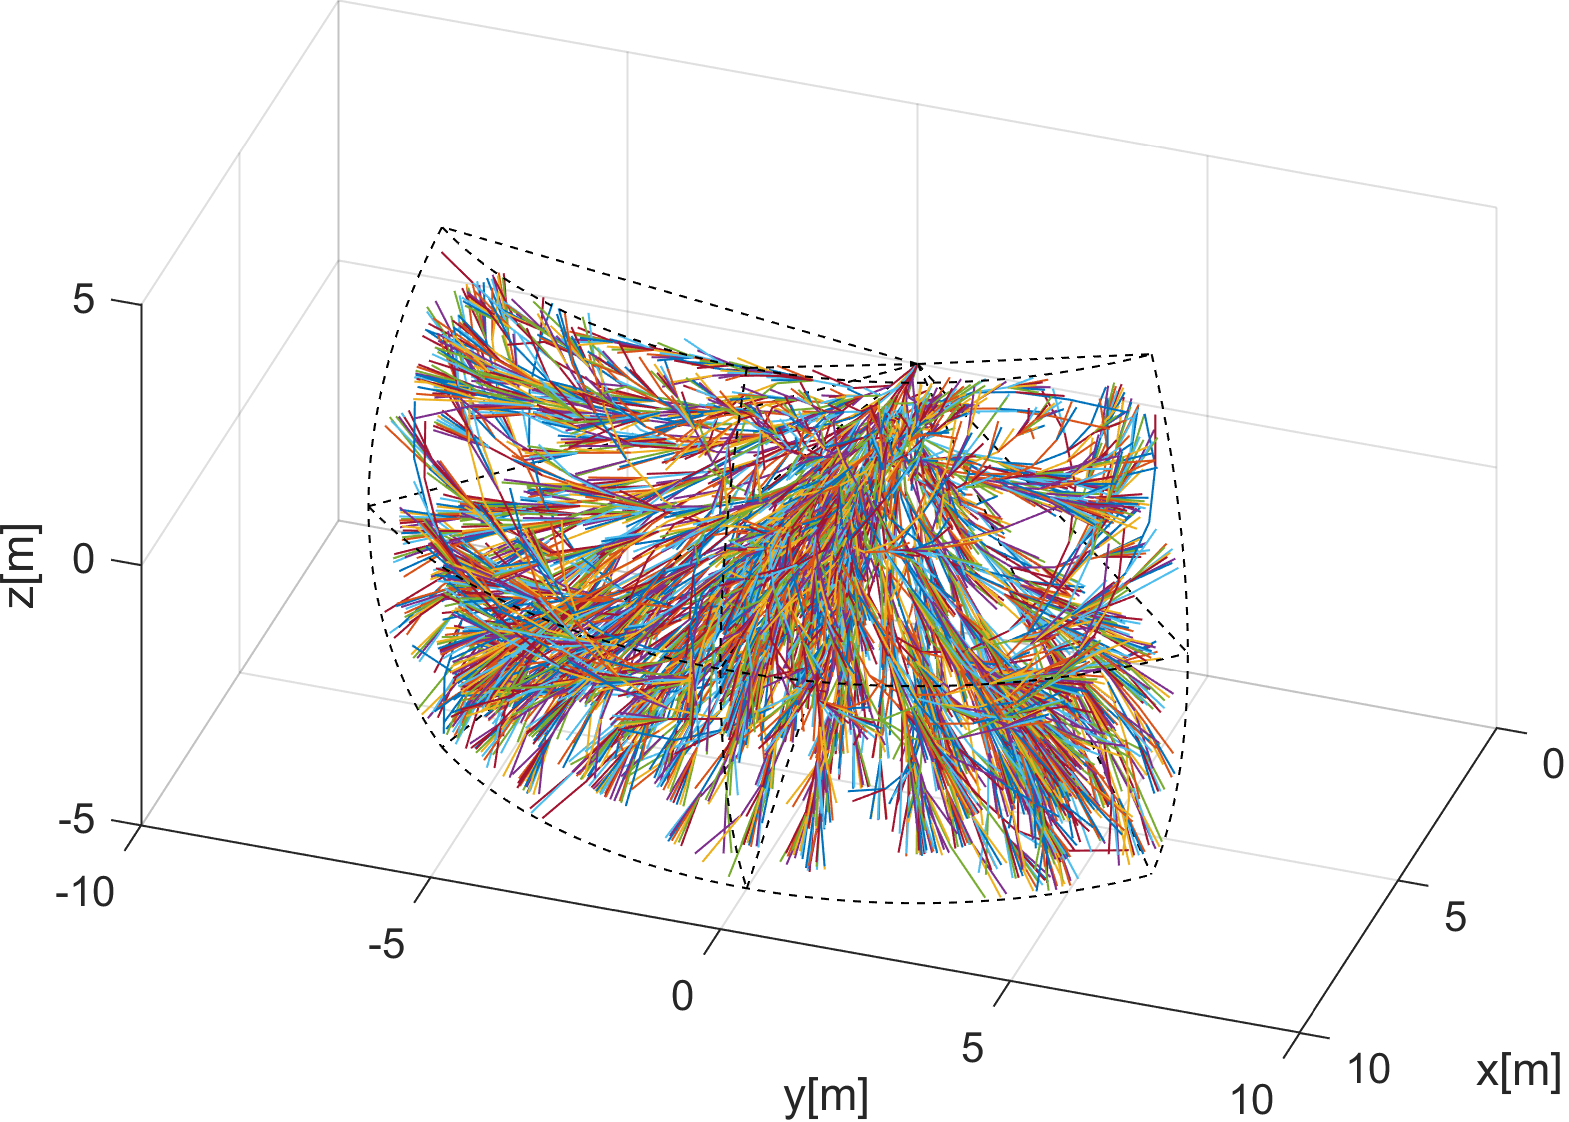
\includegraphics[width=0.9\linewidth]{\FIGDIR/NS082CoverageRS00010}
        \caption{Full.}
        \label{fig:chaoticComputed}
    \end{subfigure}
    \begin{subfigure}{0.48\textwidth}
    	\centering
        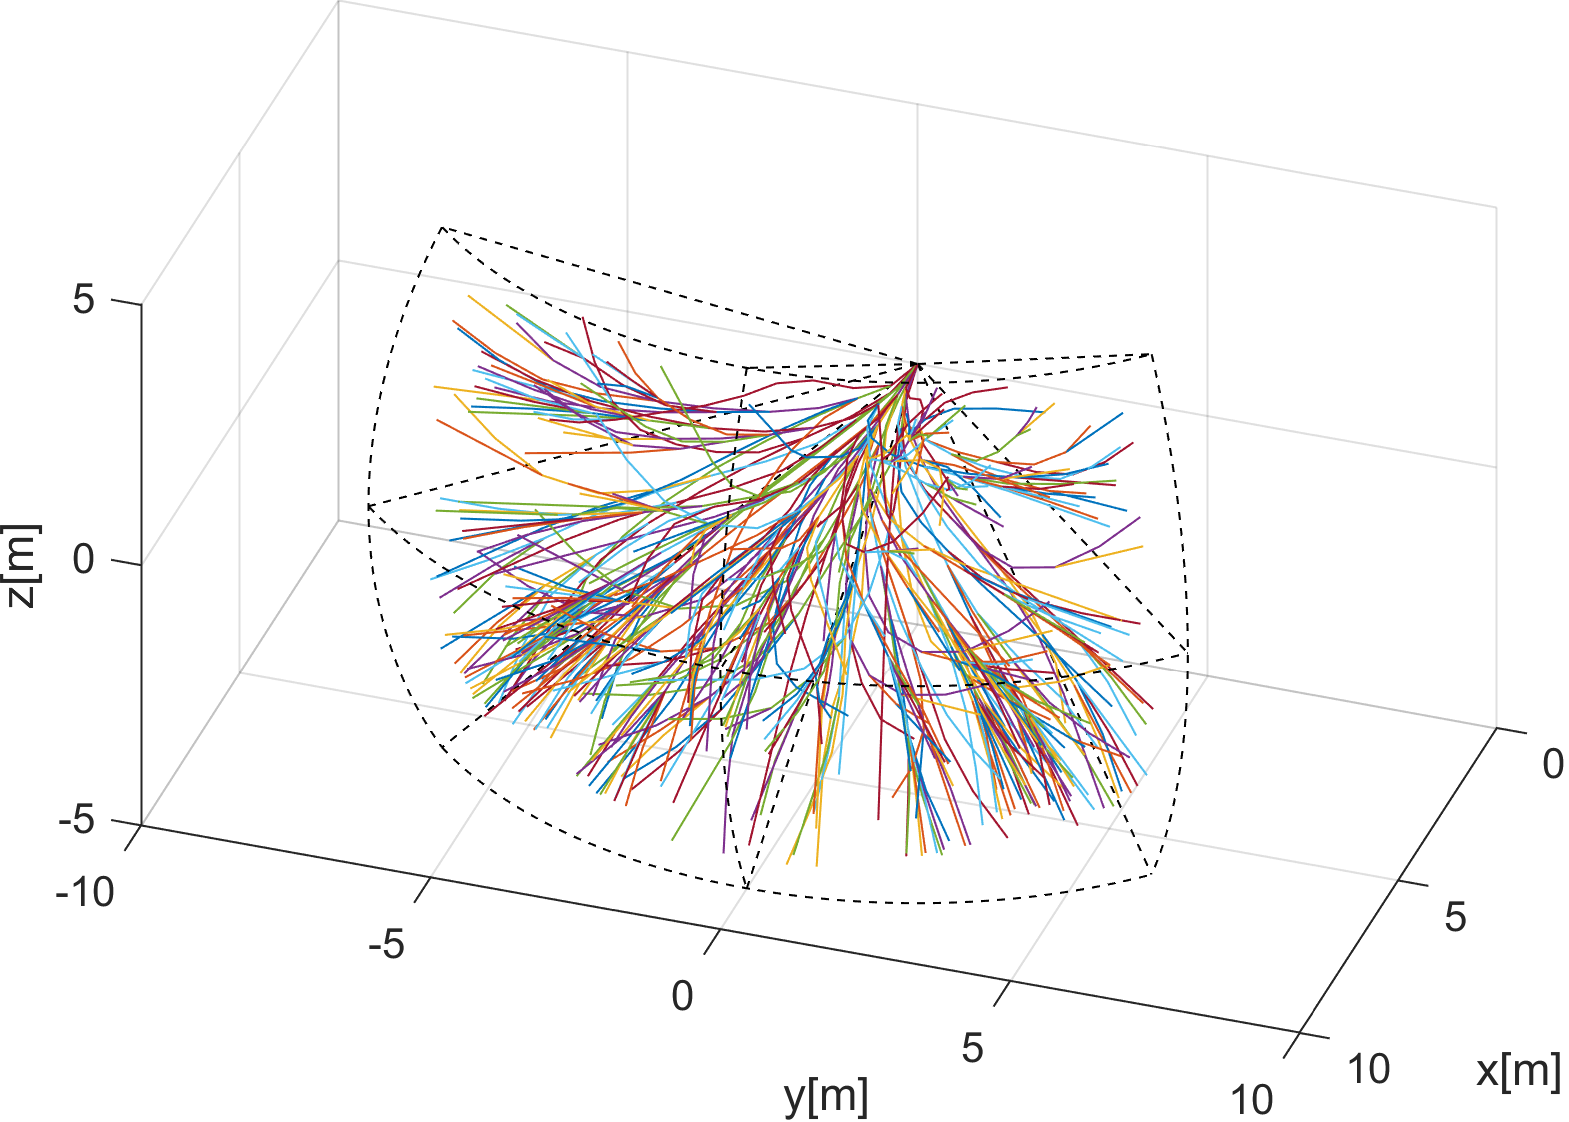
\includegraphics[width=0.9\linewidth]{\FIGDIR/NS083CoverageRSAfterPruning} 
        \caption{Pruned.}
        \label{fig:chaoticPruned}
    \end{subfigure}
    \caption{Coverage-maximizing reach set computation example.}
    \label{fig:chaoticReachSetComputationExample}
\end{figure}

\paragraph{Turn-Minimizing Reach Set} (sec. \ref{s:harmonicReachSet}) is used in \emph{Navigation Mode} for \emph{Non Controlled Airspace}. The \emph{full set} of trajectories is given in (fig. \ref{fig:harmonicComputed}). The \emph{Pruned} set of trajectories is given in (fig. \ref{fig:harmonicPruned}).

\emph{Tuning parameter} for \emph{harmonic spread ratio} was set to 9 (which implies low coverage).

\begin{figure}[H]
    \centering
    \begin{subfigure}{0.48\textwidth}
    	\centering
        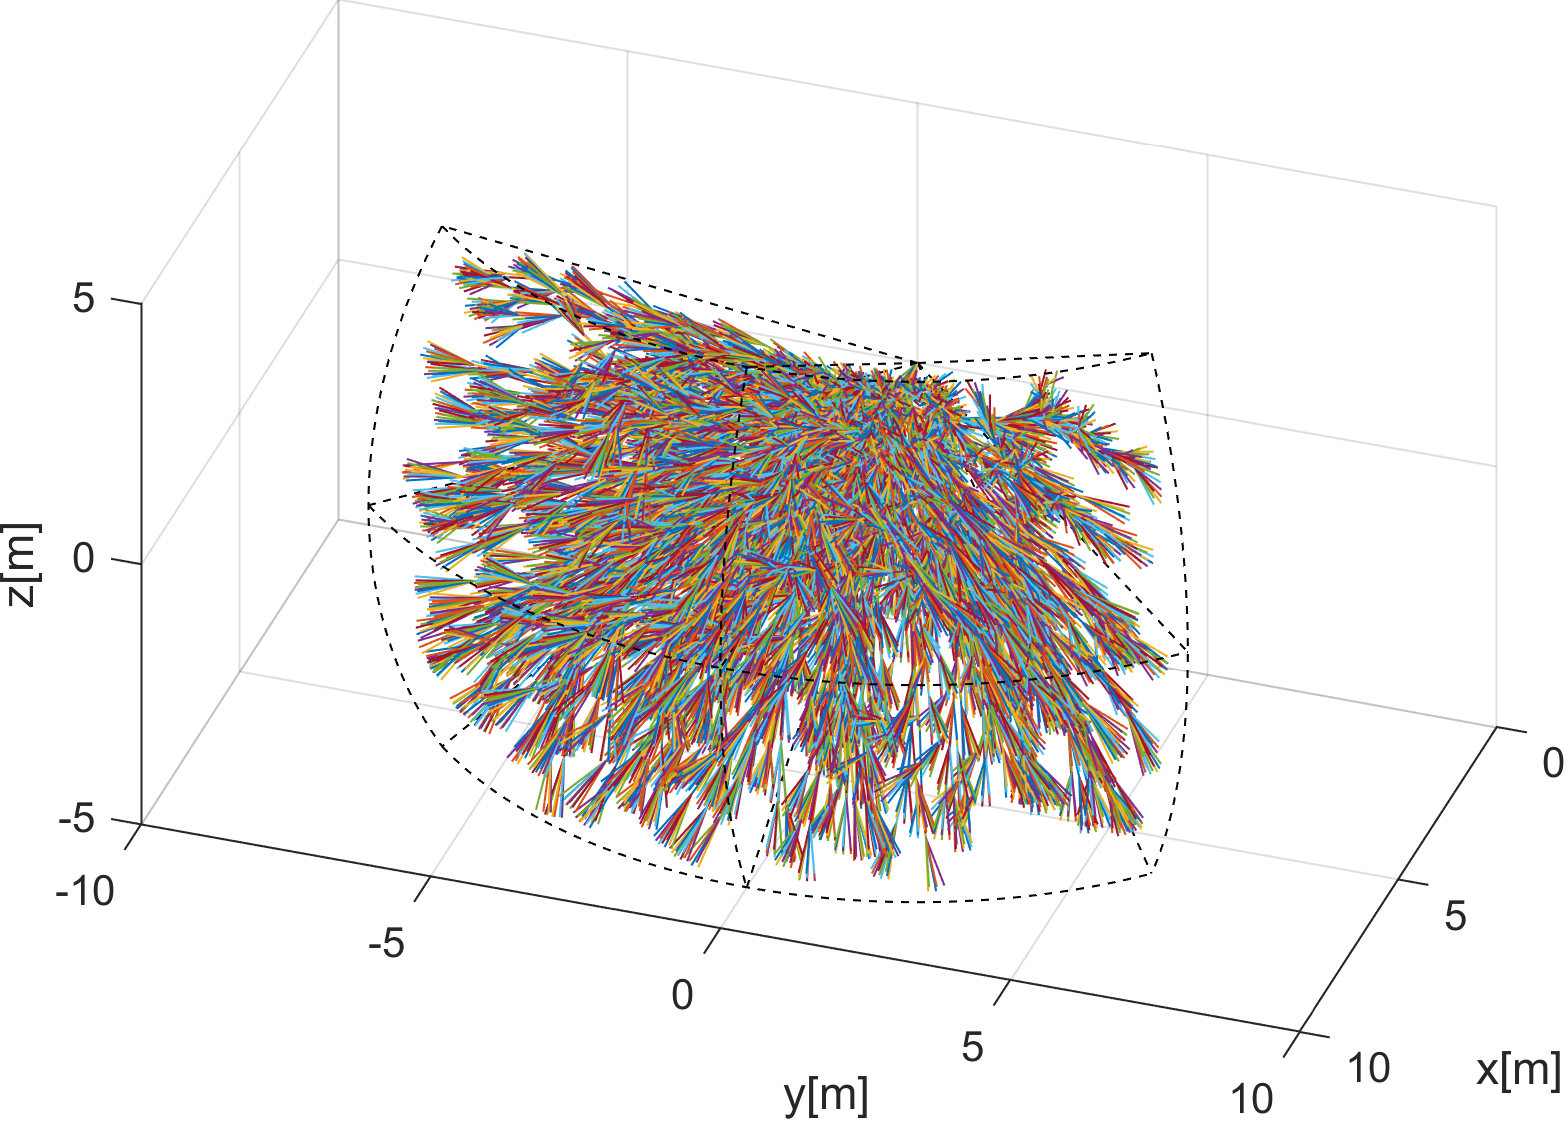
\includegraphics[width=0.9\linewidth]{\FIGDIR/NS084smoothRS00010}
        \caption{Full.}
        \label{fig:harmonicComputed}
    \end{subfigure}
    \begin{subfigure}{0.48\textwidth}
    	\centering
        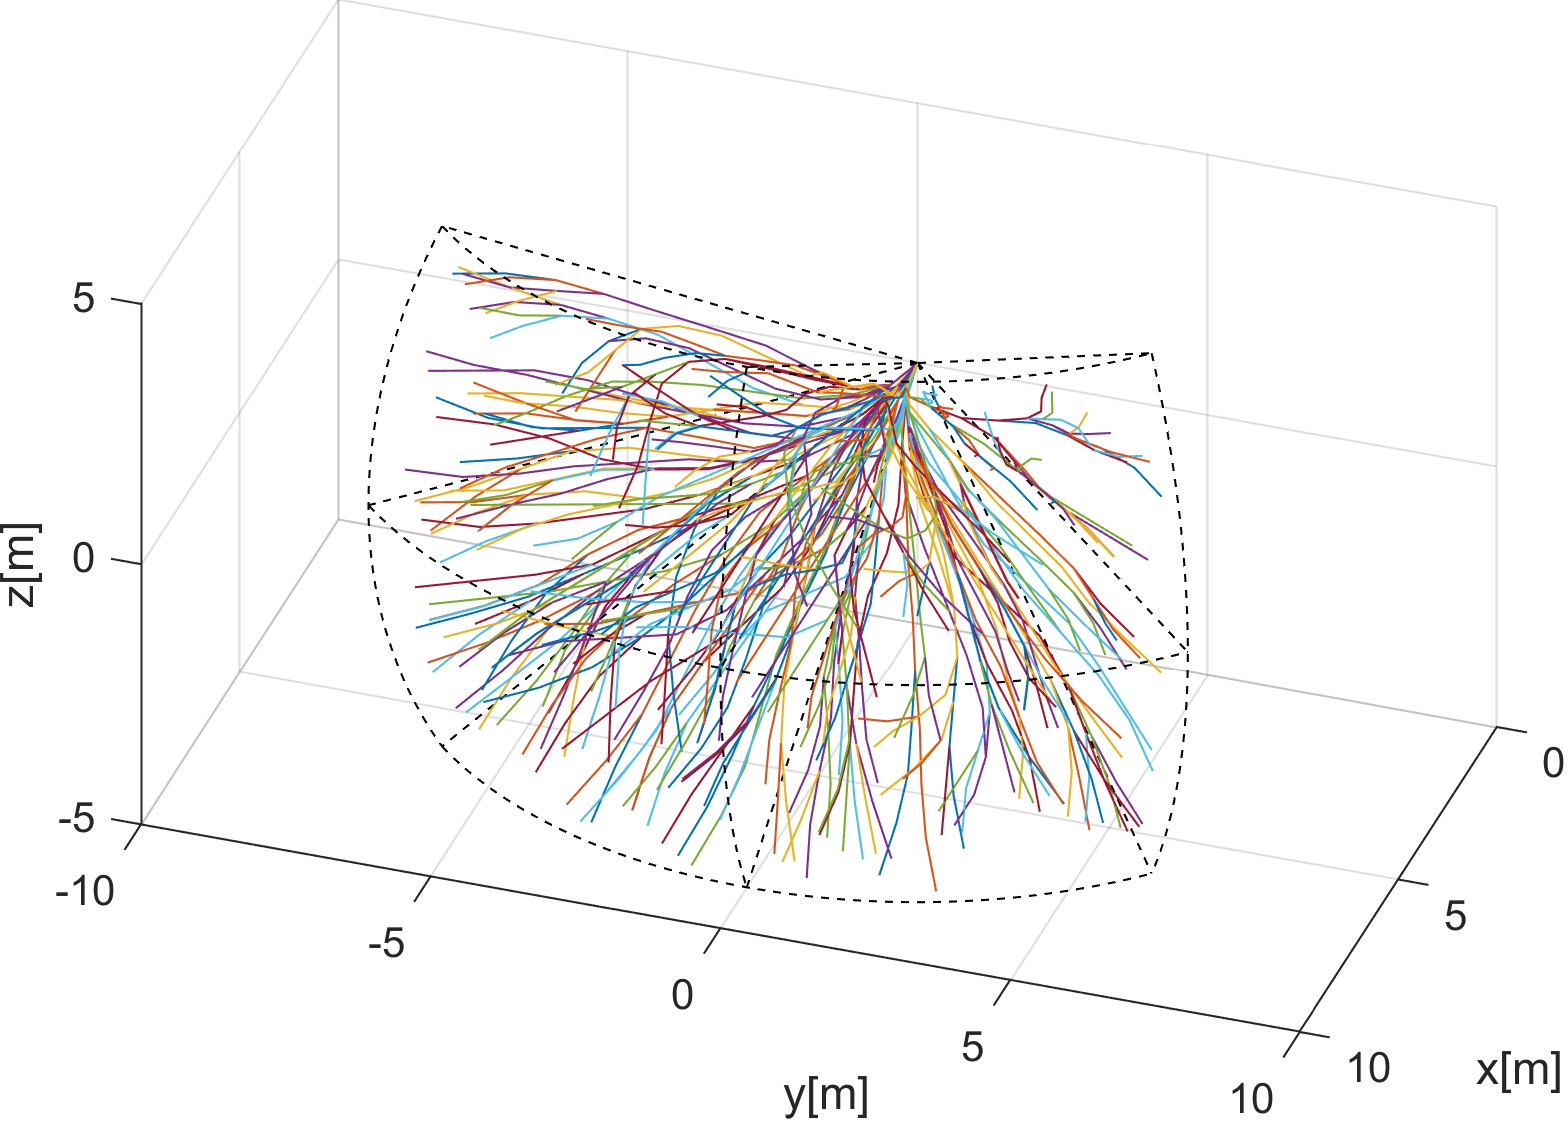
\includegraphics[width=0.9\linewidth]{\FIGDIR/NS085smoothRSAfterPruning} 
        \caption{Pruned.}
        \label{fig:harmonicPruned}
    \end{subfigure}
    \caption{Turn-minimizing reach set computation example.}
    \label{fig:harmonicReachSetComputationExample}
\end{figure}

\paragraph{Combined Reach Set} (sec. \ref{s:combinedReachSet}) is combination of \emph{Coverage-Maximizing Reach Set} (fig. \ref{fig:chaoticReachSetComputationExample}) and \emph{Turn-Minimizing Reach Set} (fig. \ref{fig:harmonicReachSetComputationExample}). The \emph{tuning parameters} are the same for the respective methods. It is used for both \emph{Emergency Avoidance} and \emph{Navigation}. 

\paragraph{ACAS-like Reach Set} (sec. \ref{s:acasReachSet}) is used in \emph{Navigation Mode} for \emph{Controlled Airspace}. The separations used are \emph{Horizontal}, \emph{Vertical}, \emph{Slash}, and, \emph{Backslash}, to give the worst possible nodes and trajectories count. The \emph{full} set of trajectories is given in (fig. \ref{fig:acasLikeComputed}). The \emph{Pruned} set of trajectories is given in (fig. \ref{fig:acasLikePruned}).

\begin{figure}[H]
    \centering
    \begin{subfigure}{0.48\textwidth}
    	\centering
        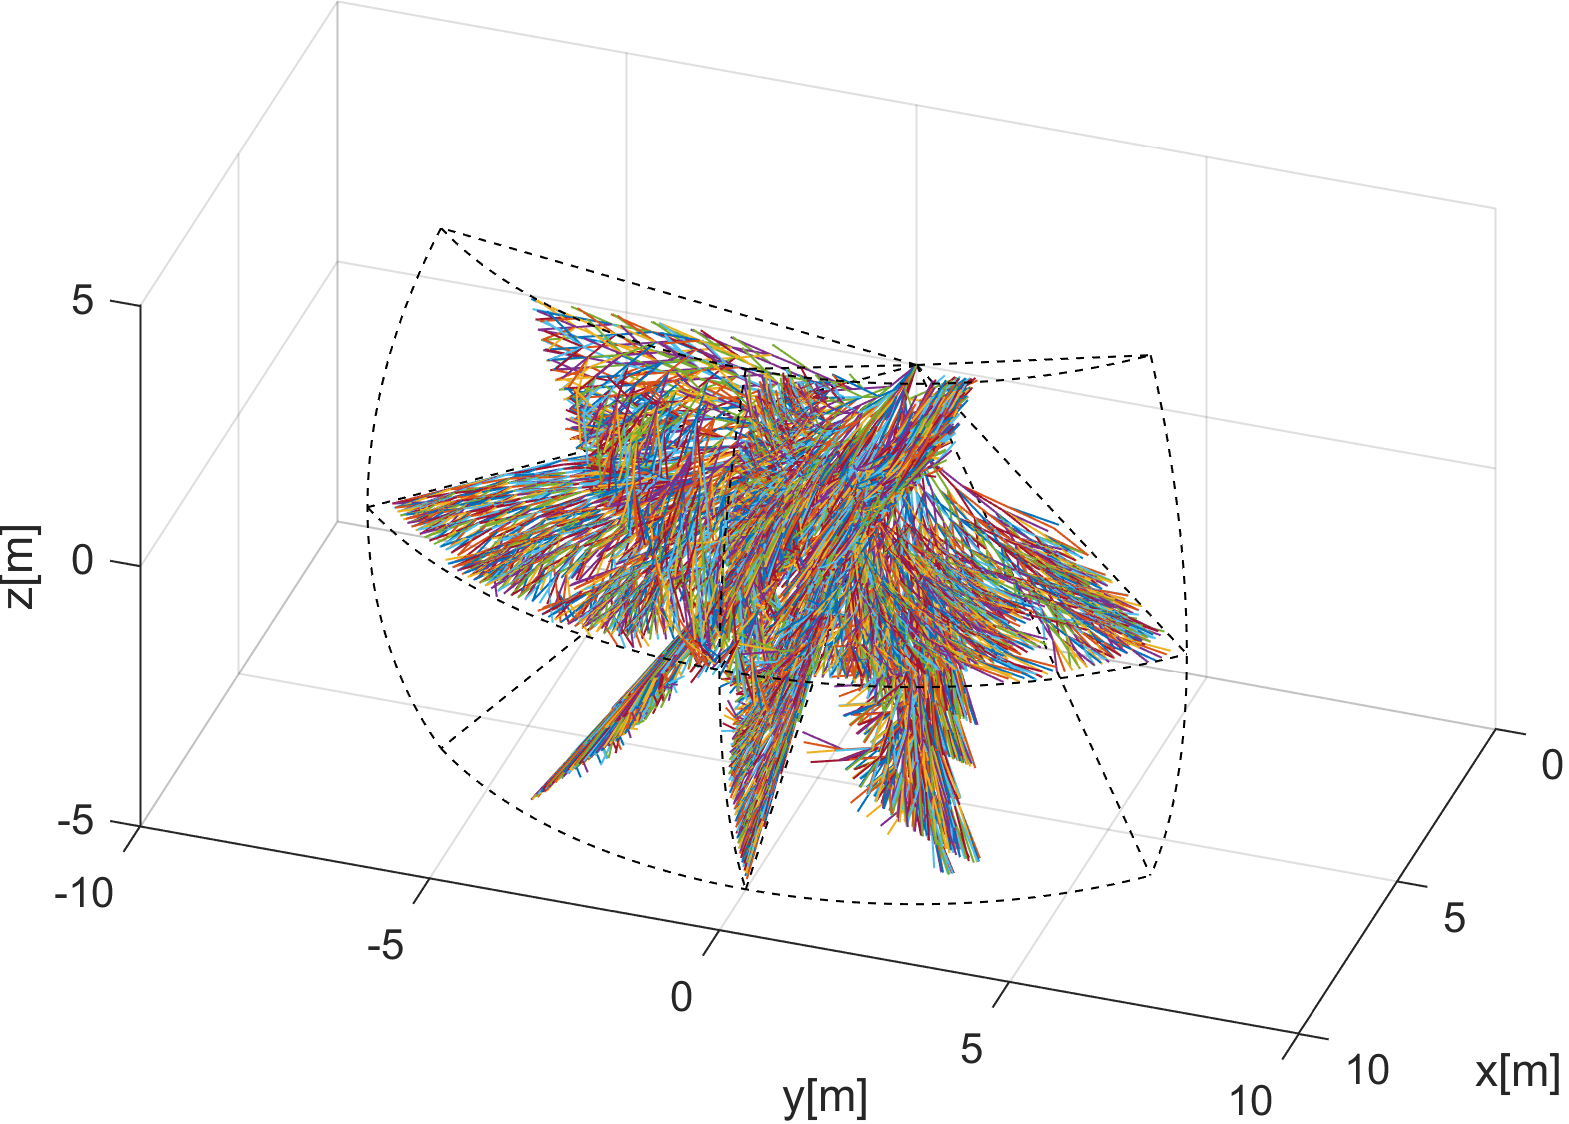
\includegraphics[width=0.9\linewidth]{\FIGDIR/NS080acasLikeRS00010}
        \caption{Full.}
        \label{fig:acasLikeComputed}
    \end{subfigure}
    \begin{subfigure}{0.48\textwidth}
    	\centering
        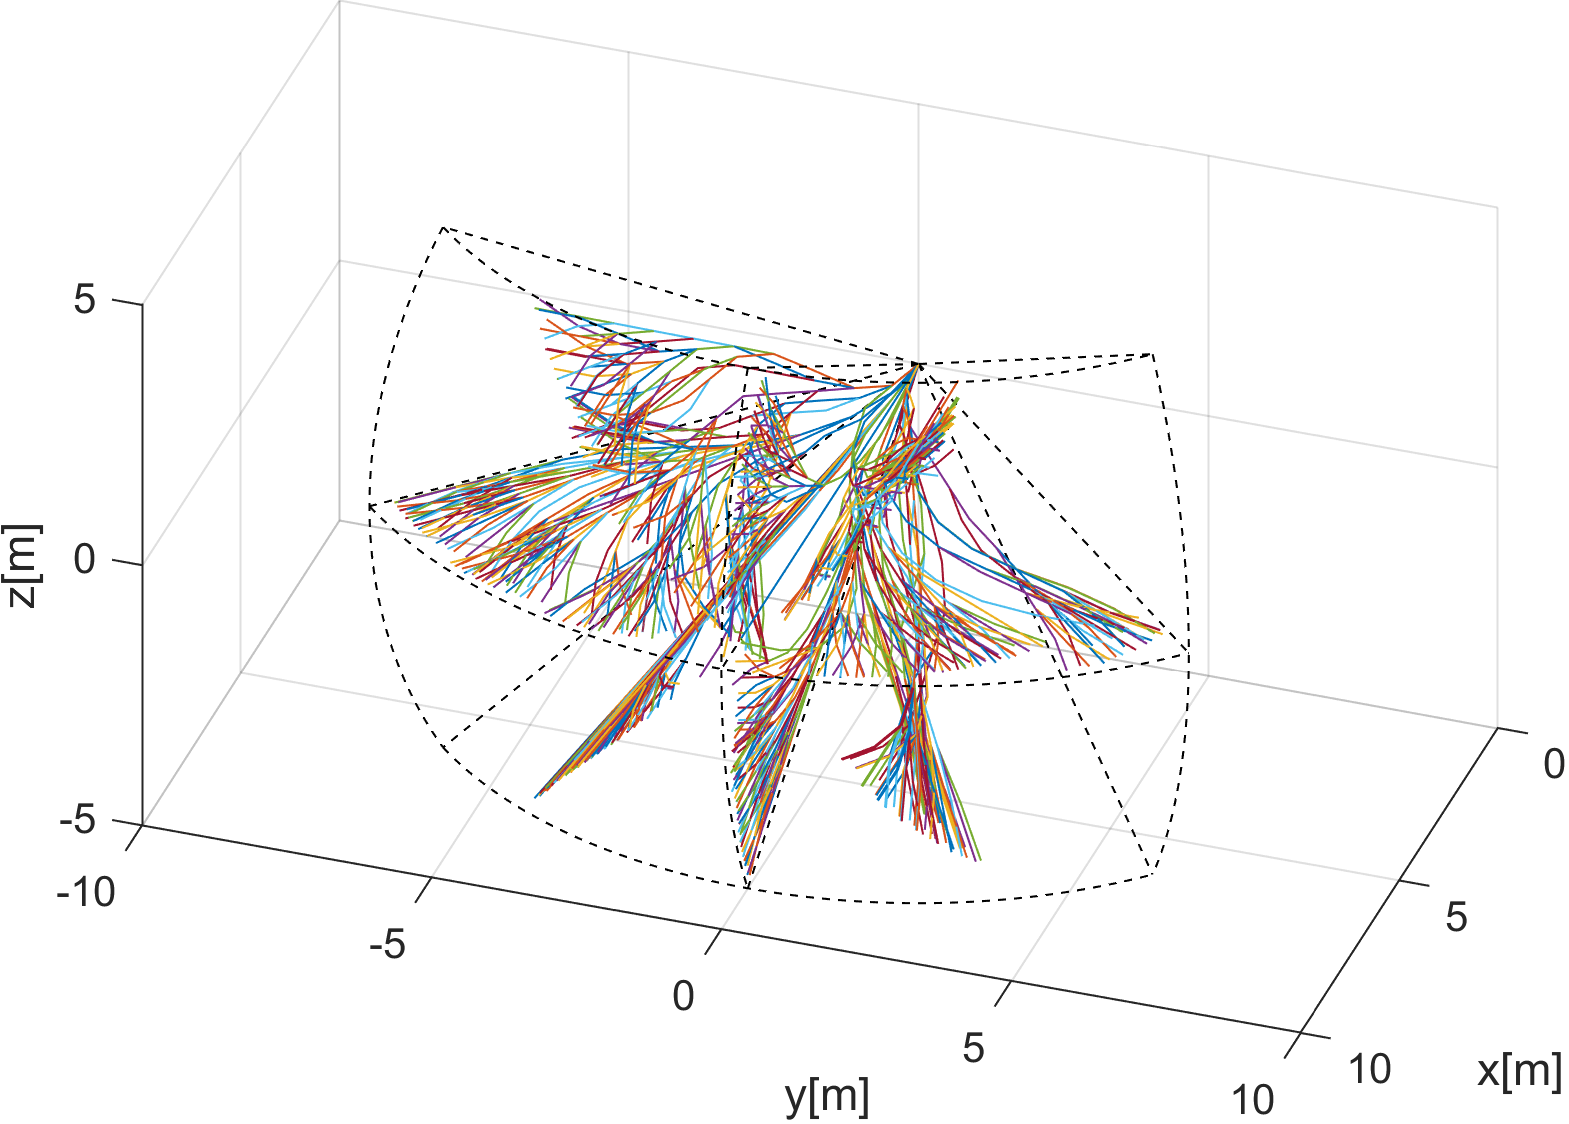
\includegraphics[width=0.9\linewidth]{\FIGDIR/NS081acasLikeRSAfterPruning} 
        \caption{Pruned.}
        \label{fig:acasLikePruned}
    \end{subfigure}
    \caption{ACAS-like reach set computation example.}
    \label{fig:acasLikeReachSetComputationExample}
\end{figure}


\paragraph{Computation Methods Performance Comparison} (tab. \ref{tab:RRMethodsPerformanceComparison})  gives overview of memory consumption and \emph{Coverage Ratio}.

\paragraph{Node count:} \emph{Full Node Count} shows how much memory it takes to compute \emph{Reach set}. \emph{Pruned Node Count} shows how much \emph{memory} is needed for storage. 

\begin{note}
    The total size of \emph{full/pruned Reach Set} depends on Node implementation. The Object-oriented prototype implementation in Matlab for example avoidance grid took up to 1 megabyte of system memory. The effective implementation would take up to 100 kilobytes.
\end{note}

\emph{Constrained expansion} (alg. \ref{alg:Wavefront Propagation}) have different selection rate, depending on the method. The survival rate directly reflects strictness of selection criteria. The rate of \emph{node pruned} is summarized in (eq.\ref{eq:NodeWasteRate})  

\begin{equation}\label{eq:NodeWasteRate}
    \begin{aligned}
        \texttt{No} & \texttt{des } \texttt{pruned}\\
        &CM-RSA   &: 78.93 \%\\
        &TM-RSA  &: 18.50 \%\\
        &ACAS-like &: 79.05 \%
    \end{aligned}
\end{equation}

\noindent The \emph{interpretation of results} for each reach set estimation method is like follow: 

\begin{enumerate}
    \item \emph{Coverage-Maximizing} - the main exploration drive  is \emph{Coverage Rate}, the \emph{Trajectory} segments are not usually smooth. For our \emph{Movement Automaton}, there is only one \emph{Smooth Movement}: Straight. Other eight are considered \emph{Chaotic Movements}. Impact of this fact is significant because $4/5$ of nodes were pruned.
    
    \item \emph{Turn-Minimizing} - the main exploration drive is \emph{Smoothness} of contained \emph{Trajectories}. The \emph{Trajectory segments} which are getting further away from \emph{cell center} are not feasible. If \emph{Smooth Movements} set size is considered, the Smooth/Chaotic movement ratio is $1/8$ for our \emph{Movement Automaton} implementation. The low node count was expected in this approach. Another Contributing factor is \emph{Trajectory Footprint Length} for uniqueness selection, which is not a tuning parameter in this method, and it is set to the most strict selection.
    
    \item \emph{ACAS-like} - the main drive is to create set consisting from \emph{multiple 2D separation planes}. The expansion method applies full movement set on the \emph{candidate node}. The \emph{Separation plane movement subset} is determining, which node will be selected for further expansion. The size of separation plane subset to the size of movement set rate is $1:3$. There are four separation planes: horizontal, vertical, slash and backslash each containing full 2D plane reach set approximation which caused high node prune rate. Nodes used rate should get lower with increasing grid size.
    
\end{enumerate}

\paragraph{Trajectories count:} \emph{Full trajectories count} shows how many \emph{leaf nodes} were existing during the calculation process without pruning. The difference between \emph{full node count} and \emph{full trajectories count} is count of inner tree nodes. 

\emph{Pruned trajectories count} shows how many \emph{leaf nodes} are used in run-time of \emph{avoidance algorithm}. The difference between \emph{pruned node count} and \emph{pruned trajectories count} shows the count of inner nodes in active reach set.

The most of \emph{waste leaf nodes} are removed during \emph{layer pruning}: function \emph{reachSet.purge- SameFootprint()} (alg. \ref{alg:Wavefront Propagation}). The \emph{Waste trajectories} or \emph{unused leaf nodes count} have significant impact. Because \emph{leaf nodes} are a side product of \emph{Node Expansion procedure} the amount of  \emph{pruned trajectories} is around 90 $\%$ regardless of the used method. The results are summarized in (eq. \ref{eq:trajectoriesWasted})

\begin{equation}\label{eq:trajectoriesWasted}
    \begin{aligned}
        \texttt{  Tr} & \texttt{ajectories } \texttt{pruned}\\
        &CM-RSA   &: 91.24 \%\\
        &TM-RSA  &: 88.21 \%\\
        &ACAS-like &: 89.43 \%
    \end{aligned}
\end{equation}

\begin{table}[H]
    \centering
    \begin{tabular}{c||c|c||c|c||c||c}
        % Header line 1
        \multirow{2}{*}{\begin{tabular}[c]{@{}c@{}}Calculation\\ method\end{tabular}} & \multicolumn{2}{c||}{Node count} & \multicolumn{2}{c||}{Trajectories} & \multirow{2}{*}{\begin{tabular}[c]{@{}c@{}}Coverage \\ ratio\end{tabular}} & \multirow{2}{*}{Parameters}\\ \cline{2-5}
        % Header line 2
        & full & pruned & full & pruned & & \\ \hline\hline
        % CM-RSA parameters
        CM-RSA  & 6727 & 1417 & 4557 & 399 & 90\% & spread:15 \\ \hline
        % TM-RSA reach set parameters
        TM-RSA & 1724 & 1405 & 1528 & 180 & 30\%  & spread:9  \\ \hline
        % Combined reach set parameters
        combined & - & 2405 & - & 435 & 95\% & \begin{tabular}[c]{@{}c@{}}CH spread:15\\ H spread:9\\ tree comb.\end{tabular}\\ \hline
        % ACASLike
        ACAS-like & 11294 & 2366 & 7437 & 786 & 74.95\% & \begin{tabular}[c]{@{}c@{}}Separations:\\ H/V/S/BS\\ Coverage pruning:\\ disabled\end{tabular} \\ 
    \end{tabular}
    \caption{\emph{Reduced reach set} computation methods performance}
    \label{tab:RRMethodsPerformanceComparison}
\end{table}

\paragraph{Coverage ratio:} (def. \ref{def:coverageRatio}) is showing how much maneuvering versatility of \emph{Reach Set}. \emph{Full Reach Set Approximation} have coverage ratio of $100$ $\%$. It is possible to construct \emph{Reference Reach Set} without constrained expansion method which contains all possible \emph{trajectory footprints}. Following observations for \emph{coverage ratio} can be made:
\begin{enumerate}
    \item \emph{Coverage-maximizing} reach set estimation method by design select \emph{Nodes} which have the high probability of \emph{trajectory footprint} diversification. The high coverage ratio was achieved at values around 90 $\%$.
    
    \item \emph{Turn-Minimizing} reach set estimation method by design selects most smooth trajectories which cause low \emph{trajectory footprint} diversity. The fairly high coverage ratio of $30$ $\%$ has been achieved.
    
    \item \emph{Combined} reach set estimation method takes two reach set and combines their trajectory trees into a single trajectory tree. It is given that \emph{Coverage ratio} will achieve at least maximal coverage ratio of original reach sets. Harmonic reach set supplemented narrow smooth trajectories which were throw away previously; this increased overall \emph{coverage ratio} to $95$ $\%$. 
    
    \item \emph{ACAS-like} reach set estimation method contained four separation planes, which caused that it was similar to \emph{Coverage-Maximizing Reach Set Approximation} for given \emph{Avoidance Grid}, concerning of performance. The coverage ratio For 2D plane was $100$ $\%$.
\end{enumerate}


    %Observations moved to Conclusion - no longer in use
    %\section{(W) Simulation Observations Summary}\label{sec:SimulationObservationsSummary}
    \noindent Use summary of this section in Conclusion and future work on specific 

\subsection{(W) Static Obstacles Avoidance}\label{sec:staticObstacleAvoidanceSummary}
    \noindent TODO: main points of building, slalom, maze scenarios - link artifacts and performance criteria

\subsection{(W) Constraints Avoidance}\label{sec:constraintAvoidanceSummary}
    \noindent TODO constraints main point, main loop processing, breach chance ? etc...
    
\subsection{(W) Unsupervised Intruder Avoidance}\label{sec:unsupervisedIntruderAvoidance}
    \noindent TODO emergency intruder avoidance emphasis navigation, Emergency avoidance contribution main points

\subsection{(W) Supervised (UTM) Intruder Avoidance}\label{sec:supervisedIntruderAvoidance}
    \noindent TODO UTM contribution main points
    
 

%% This adds a line for the Bibliography in the Table of Contents.
\addcontentsline{toc}{chapter}{Bibliography}
%% *** Set the bibliography style. ***
%% (change according to your preference/requirements)
%\bibliographystyle{plain}
%% *** Set the bibliography file. ***
%% ("thesis.bib" by default; change as needed)
\bibliography{thesis}

%% *** NOTE ***
%% If you don't use bibliography files, comment out the previous line
%% and use \begin{thebibliography}...\end{thebibliography}.  (In that
%% case, you should probably put the bibliography in a separate file and
%% `\include' or `\input' it here).

\end{document}
